\section{蒙特卡洛模拟与统计验证}\label{sec:simulation}
\subsection{独立排列、估计量与区间}
理论计算采用精确组合数与有理数；模拟则独立生成带编号实体牌的随机排列，
从前$n$张判断$I$，并读取随后$h$张计算$X$、$Y$。
107组不同的“牌组、$n$、$h$”配置各运行$m=200\,000$次，
基准另做$1\,000\,000$次独立复验。
伪随机生成器为NumPy的PCG64，根种子为20261114，
不同配置、复验和收敛实验按独立派生流执行。
同一排列上的多个前缀统计量具有相关性。

设第$r$次试验结果为$(I_r,Y_r)$，成功数
$K=\sum_{r=1}^m I_r$。使用
\begin{equation}\label{eq:estimators}
\widehat p=\frac Km,\qquad
\overline Y=\frac1m\sum_{r=1}^mY_r,\qquad
\widehat\mu=\frac1K\sum_{r:I_r=1}Y_r
\end{equation}
估计启动概率、总体均值与条件均值。
条件指标以成功次数$K$作为样本量。
所有配置的联合分布均核对$\sum_xJ_x=p$；
条件与总体PMF分别核对归一性，并检验式\eqref{eq:total-moments}。
当$p=0$时，总体收益为0，条件指标按未定义处理。

启动比例采用Wilson区间\cite{wilson}。
令$z_{0.975}\approx1.96$为标准正态分位数，则区间为
\begin{equation}\label{eq:wilson}
\frac{\widehat p+z_{0.975}^2/(2m)
\ \pm\ z_{0.975}
\sqrt{\widehat p(1-\widehat p)/m+z_{0.975}^2/(4m^2)}}
{1+z_{0.975}^2/m}.
\end{equation}
总体均值采用$\overline Y\pm z_{0.975}s_Y/\sqrt m$，
其中$s_Y^2$是分母为$m-1$的无偏样本方差；
条件均值区间相应使用成功样本标准差与$\sqrt K$。
有界收益保证有限方差，大数定律给出估计收敛，
中心极限定理给出这些均值区间的渐近依据\cite{blitzstein}。

\subsection{基准验证与抽样误差}
表\ref{tab:validation}保留两次独立运行。
20万次主实验中，启动率与总体均值的95\%区间未覆盖理论值，
对应标准化误差约为$-3.008$与$-3.279$；
条件均值区间覆盖理论值。
100万次独立复验的三个区间均覆盖理论值。
复验使用另一条独立随机流。

\begin{table}[htbp]
\centering\small
\caption{基准精确理论与独立排列模拟；概率用Wilson区间，均值用CLT区间}\label{tab:validation}
\setlength{\tabcolsep}{6pt}
\begin{tabular}{lrrrrr}
\toprule
指标 & 排列次数 & 条件样本量$K$ & 精确理论 & 模拟估计 & 95\%置信区间 \\
\midrule
$p$ & 200,000 & --- & 0.098814 & 0.096825 & [0.095537, 0.098129] \\
$p$ & 1,000,000 & --- & 0.098814 & 0.098648 & [0.098065, 0.099234] \\
$\mu$ & 200,000 & 19,365 & 16.914286 & 16.846476 & [16.742636, 16.950316] \\
$\mu$ & 1,000,000 & 98,648 & 16.914286 & 16.880464 & [16.834366, 16.926562] \\
$\mathbb E(Y)$ & 200,000 & --- & 1.671372 & 1.631160 & [1.607123, 1.655197] \\
$\mathbb E(Y)$ & 1,000,000 & --- & 1.671372 & 1.665224 & [1.654361, 1.676087] \\
\bottomrule
\end{tabular}

\end{table}

95\%置信区间具有重复抽样意义，基准主实验的偏差展示了单次区间的随机性。
在101个非退化配置中，启动率与总体均值的标准化误差绝对值超过1.96的配置
分别为5组与4组。精确计数、全排列核查与随机模拟共同检验了数值实现。

为考察样本量对精度的影响，分别在
$m=2\,000,10\,000,50\,000,200\,000$下独立重复30次，
计算估计误差的均方根（RMSE）。
启动率与总体均值的理论标准误为
\begin{equation}\label{eq:mc-scale}
\operatorname{SE}(\widehat p)=\sqrt{\frac{p(1-p)}m},\qquad
\operatorname{SE}(\overline Y)=\sqrt{\frac{\V(Y)}m}.
\end{equation}
图\ref{fig:convergence}中，实测RMSE与理论尺度相符：
总体均值RMSE由0.117652降至0.012047，理论标准误由0.124165降至0.012416。
样本量扩大5倍时，理论标准误缩小为原来的$1/\sqrt5$；
重复实验的RMSE围绕相应尺度变化。

\begin{figure}[htbp]
\centering
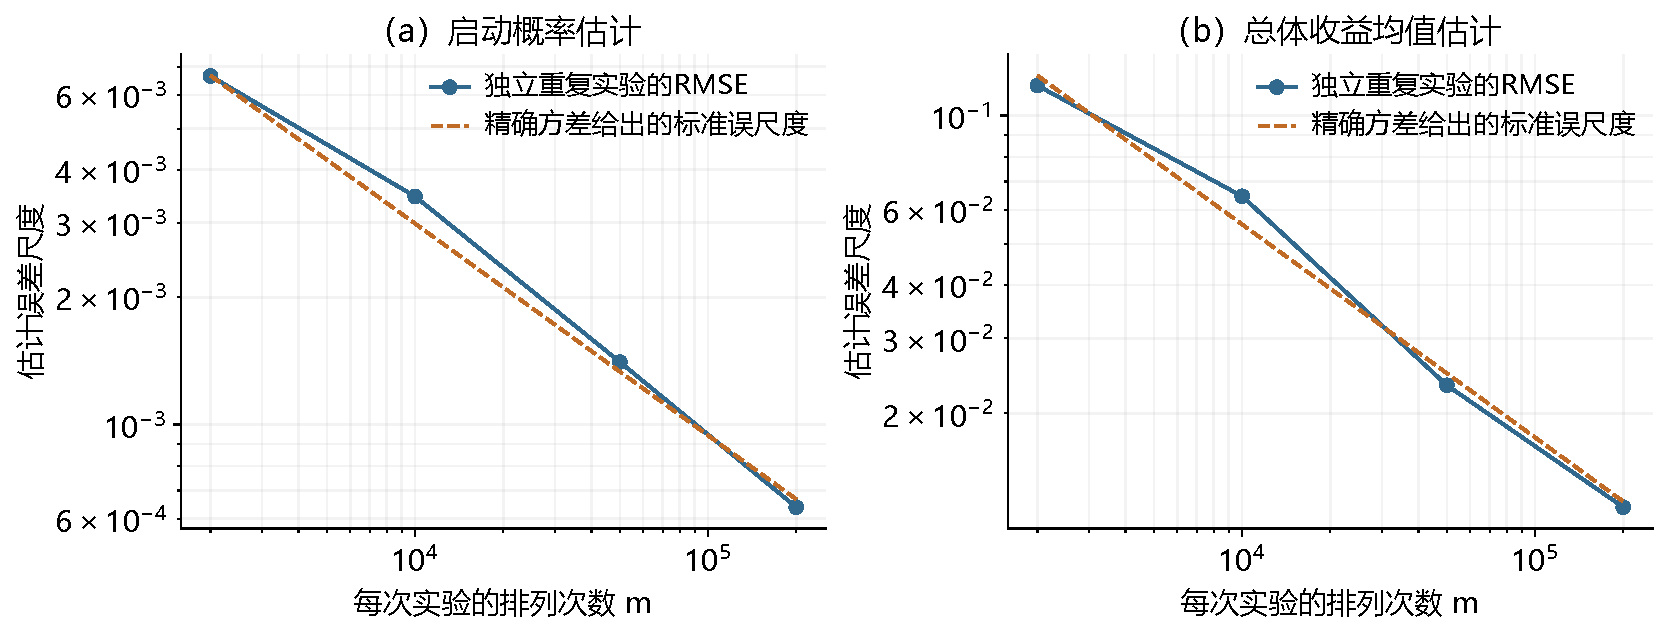
\includegraphics[width=\linewidth]{09_convergence.pdf}
\caption{不同样本量下各30次独立重复的RMSE与精确方差给出的标准误尺度；
双对数坐标中的理论斜率为$-1/2$。}\label{fig:convergence}
\end{figure}

\FloatBarrier
\section{结论与展望}
本文用联合可及性与条件回报两个层次，刻画了有限随机卡组的协同收益。
容斥与尾和公式给出组件见齐概率和首次见齐时间；
有限前缀的顺序计数进一步表明，组件齐全与满足特定先后要求是不同事件。
同洗牌的条件超几何混合保留了前后阶段的组成依赖，
使条件收益与总体收益可以在统一样本空间中计算。

固定牌组规模时，交换性把条件收益均值与方差分别化为一次式与二次式，
并确定条件方差在普通非攻击牌数为9时最大。
全方差分解揭示，基准总体波动主要来自成功与失败两类条件均值的差异。
明确区分增删与替换后，增加普通非攻击牌所产生的条件回报提升，
可以与组件可及性下降同时发生；总体期望由两者共同决定。
这些结果说明，稳定性需要结合事件概率、条件分布与操作成本解释。

后续研究可以引入抽牌反馈、重新洗牌、能量约束和出牌策略，
建立动态状态转移模型，考察卡组构筑对启动效率与消耗收益的影响。
